78. $f(x)=\cfrac{|x^2-3x|(x+1)}{x}=\cfrac{|x||x-3|(x+1)}{x}=\begin{cases} x^2-2x-3,\ x\geqslant3,\\ -x^2+2x+3,\ 0<x<3,\\ x^2-2x-3,\ x<0.\end{cases}$
$$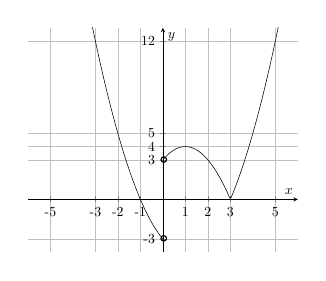
\begin{tikzpicture}[scale=0.5]
\begin{axis}[
    axis lines = middle,
    grid=major,
    legend pos={south west},
    xlabel = {$x$},
    %xlabel style={below right},
    ylabel = {$y$},
    ymin=-4,
    ymax=13,
    xmin=-6,
    xmax=6,
    xtick={-5,-3,-2,-1,1,2,3,5},
    xticklabels={-5,-3,-2,-1,1,2,3,5},
    ytick={12,3,-3,4,5},
    yticklabels={12,3,-3,4,5},
                  ]
	\addplot[domain=-6:0, samples=100, color=black] {-abs(x-3)*(x+1)};
    \addplot[domain=0:6, samples=100, color=black] {abs(x-3)*(x+1)};
        %\addplot[domain=2.01:6, samples=100, color=black] {2/(2-x)};
   % \addplot[domain=-3:3, samples=100, color=black] {-x};
     %\addlegendentry{$\text{Рис. 1}$};
\end{axis}
\draw (3.45,2.35) circle (2pt);
\draw (3.45,0.35) circle (2pt);
%\draw (3.45,2.55) circle (2pt);
\end{tikzpicture}$$
